%%%%%%%%%%%%%%%%%%%%%%%%%%%%%%%%%%%%%%%%%
% Beamer Presentation
% LaTeX Template
% Version 1.0 (10/11/12)
%
% This template has been downloaded from:
% http://www.LaTeXTemplates.com
%
% License:
% CC BY-NC-SA 3.0 (http://creativecommons.org/licenses/by-nc-sa/3.0/)
%
%%%%%%%%%%%%%%%%%%%%%%%%%%%%%%%%%%%%%%%%%

%----------------------------------------------------------------------------------------
%   PACKAGES AND THEMES
%----------------------------------------------------------------------------------------

\documentclass{beamer}

\mode<presentation> {

% The Beamer class comes with a number of default slide themes
% which change the colors and layouts of slides. Below this is a list
% of all the themes, uncomment each in turn to see what they look like.

%\usetheme{default}
%\usetheme{AnnArbor}
%\usetheme{Antibes}
%\usetheme{Bergen}
\usetheme{Berkeley}
%\usetheme{Berlin}
%\usetheme{Boadilla}
%\usetheme{CambridgeUS}
%\usetheme{Copenhagen}
%\usetheme{Darmstadt}
%\usetheme{Dresden}
%\usetheme{Frankfurt}
%\usetheme{Goettingen}
%\usetheme{Hannover}
%\usetheme{Ilmenau}
%\usetheme{JuanLesPins}
%\usetheme{Luebeck}
%\usetheme{Madrid}
%\usetheme{Malmoe}
%\usetheme{Marburg}
%\usetheme{Montpellier}
%\usetheme{PaloAlto}
%\usetheme{Pittsburgh}
%\usetheme{Rochester}
%\usetheme{Singapore}
%\usetheme{Szeged}
%\usetheme{Warsaw}

% As well as themes, the Beamer class has a number of color themes
% for any slide theme. Uncomment each of these in turn to see how it
% changes the colors of your current slide theme.

%\usecolortheme{albatross}
%\usecolortheme{beaver}
%\usecolortheme{beetle}
%\usecolortheme{crane}
%\usecolortheme{dolphin}
%\usecolortheme{dove}
%\usecolortheme{fly}
%\usecolortheme{lily}
%\usecolortheme{orchid}
%\usecolortheme{rose}
%\usecolortheme{seagull}
%\usecolortheme{seahorse}
%\usecolortheme{whale}
%\usecolortheme{wolverine}

%\setbeamertemplate{footline} % To remove the footer line in all slides uncomment this line
%\setbeamertemplate{footline}[page number] % To replace the footer line in all slides with a simple slide count uncomment this line

%\setbeamertemplate{navigation symbols}{} % To remove the navigation symbols from the bottom of all slides uncomment this line
}

\usepackage{graphicx} % Allows including images
\usepackage{booktabs} % Allows the use of \toprule, \midrule and \bottomrule in tables
\usepackage[T1]{fontenc} % So LaTeX doesn't complain about > and < symbols
\usepackage{color}
\usepackage{listings}
\usepackage{lmodern}
\usepackage{amsmath}  % AMS packages for mathematical symbols
\usepackage{amsfonts}
\usepackage{amssymb}

%----------------------------------------------------------------------------------------
%   TITLE PAGE
%----------------------------------------------------------------------------------------

\title[Chapter 1]{Learning SQL: Chapter 1 } % The short title appears at the bottom of every slide, the full title is only on the title page

\author{Jimmy Nguyen} % Your name
\institute[UCSF] % Your institution as it will appear on the bottom of every slide, may be shorthand to save space
{
Francis I. Proctor Foundation \\ % Your institution for the title page
\medskip
\textit{hieu.nguyen@ucsf.edu} % Your email address
}
\date{\today} % Date, can be changed to a custom date

\begin{document}
\lstset{ % Set code-block style
	language=SQL, % turn SQL keyword highlighting on
	frame=single, % draw border delineating code
	basicstyle=\small,          % make font small to ensure fits on slide
	commentstyle=\color{gray}, % comments in gray
	keywordstyle=\color{blue}, % keywords in blue
	stringstyle=\color{red}    % strings in red 
} 

\begin{frame}
\titlepage % Print the title page as the first slide
\end{frame}

\begin{frame}
\frametitle{Overview} % Table of contents slide, comment this block out to remove it
\tableofcontents % Throughout your presentation, if you choose to use \section{} and \subsection{} commands, these will automatically be printed on this slide as an overview of your presentation
\end{frame}

%----------------------------------------------------------------------------------------
%   PRESENTATION SLIDES
%----------------------------------------------------------------------------------------


%------------------------------------------------
\section{Introduction to Databases}
%------------------------------------------------

%SLIDE-------------------------------------------
\begin{frame}
\frametitle{Relational model}
\begin{block}{Big Idea}
	Redundant data is used to link records in different tables
\end{block}

Typically, redundant data are some kind of identifier
\begin{itemize}
	\item Patient ID
	\item OD or OS
	\item Study site number
\end{itemize}
\end{frame}
%END-SLIDE---------------------------------------

%SLIDE-------------------------------------------
\begin{frame}
\frametitle{Example of relational database}
\begin{figure}
	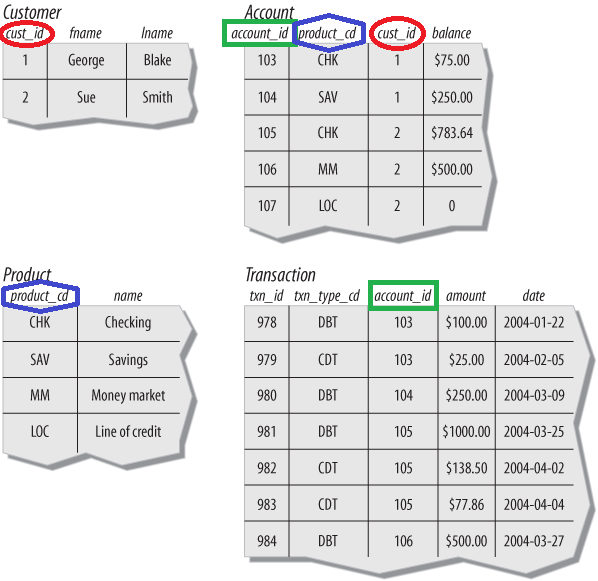
\includegraphics[width=0.6\textwidth]{Figures/figure1-3.png}
	\caption{Notice redundant columns linking each table...}
\end{figure}
\end{frame}
%END-SLIDE---------------------------------------

%SLIDE-------------------------------------------
\begin{frame}
\frametitle{"Key" Terms ;)}

\begin{description}[align=left]
	\item[primary key] column(s) of unique identifiers for rows
	\item[foreign key] column(s) together that identify a single row in another table
	\item[result set] a nonpersistent table, generally an SQL query result

\end{description}

\vspace*{1em}

\textbf{Important:} Primary keys should never be allowed to change!
\end{frame}
%END-SLIDE---------------------------------------

%SLIDE-------------------------------------------
\begin{frame}
\frametitle{Redundant information typically just identifiers}

\begin{block}{Normalization}
	Each independent piece of information is in only one place
\end{block}

Example: a patient's address changes
\begin{itemize}
	\item Ideally, we change address entry for patient with \texttt{patient\_id} 105 in the table \textbf{addresses}
	\item No other table should contain addresses
	\item Idea: carefully design database to avoid unnecessary redundancies and ensure maintainability
\end{itemize}

\end{frame}
%END-SLIDE---------------------------------------

%------------------------------------------------
\section{What is SQL?}
%------------------------------------------------

%SLIDE-------------------------------------------
\begin{frame}
\frametitle{So what is SQL?}
\begin{itemize}
	\item Pronounced S-Q-L or \textit{sequel}
	\item Used to manipulating data in relational databases
	\item Went from DSL/Alpha -> SQUARE -> SEQUEL -> SQL
	\item Apparently, SQL doesn't actually stand for anything
	\begin{itemize}
		\item People insist on "Structured Query Language"
	\end{itemize}
	\item SQL has ANSI standards which are periodically updated (currently SQL:2016)
\end{itemize}
\end{frame}
%END-SLIDE---------------------------------------

%SLIDE-------------------------------------------
\begin{frame}
\frametitle{SQL is non-procedural}
\begin{itemize}
	\item You define the results through queries, and queries are sent to an \textit{optimizer} that decides how to execute the query
	\item SQL cannot create complete applications, and is typically integrated into other languages
	\item Database administrators can influence optimizer behavior through tweaking \textit{optimizer hints}, but most end-users shouldn't care too much about this
	
\end{itemize}
\end{frame}
%END-SLIDE---------------------------------------

%SLIDE-------------------------------------------
\begin{frame}
\frametitle{SQL Statement Classes}
\begin{description}[align=left]
	\item[schema statements] define data structures stored in database
	\item[\textbf{data statements}] manipulate data structures
	\item[transaction statements] begin, end, and roll back transactions
\end{description}

Note: transactions statements will be covered in Ch 12; book focuses on data statements
\end{frame}
%END-SLIDE---------------------------------------

%SLIDE-------------------------------------------
\begin{frame}[fragile]
\frametitle{Example: SQL Schema Statement}
\begin{figure}
\begin{lstlisting}
CREATE TABLE corporation
 (corp_id SMALLINT,
  name VARCHAR(30),
  CONSTRAINT pk_corporation PRIMARY KEY (corp_id)
 );
\end{lstlisting}
\caption{Create table with two columns, \textbf{corp\_id} and \textbf{name}}
\end{figure}
\end{frame}
%END-SLIDE---------------------------------------

%SLIDE-------------------------------------------
\begin{frame}[fragile]
\frametitle{Example: SQL Data Statement}
\begin{figure}
\begin{lstlisting}
INSERT INTO corporation (corp_id, name)
VALUES (27, 'Acme Paper Corporation');
\end{lstlisting}
\caption{Insert row into \textbf{corporation} table with \textbf{corp\_id}=\textbf{27} and \textbf{name}=\textbf{Acme Paper Corporation}}
\end{figure}
\end{frame}
%END-SLIDE---------------------------------------

%SLIDE-------------------------------------------
\begin{frame}[fragile]
\frametitle{Example: SQL \texttt{select} Statement}
\begin{figure}
\begin{lstlisting}
mysql< SELECT name
	-> FROM corporation
	-> WHERE corp_id= 27;
+------------------------+
| name                   |
+------------------------+
| Acme Paper Corporation |
+------------------------+
\end{lstlisting}
\caption{Retrieve the name in the table \textbf{corporation} with \textbf{corp\_id} 27}
\end{figure}
\end{frame}
%END-SLIDE---------------------------------------

%SLIDE-------------------------------------------
\begin{frame}[fragile]
\frametitle{Basic SQL query structure}
\begin{figure}
\begin{lstlisting}
SELECT /* one or more things */ ...
FROM /* one or more places */ ...
WHERE /* one or more conditions apply */ ...
\end{lstlisting}
\caption{Most SQL queries will have at least three clauses}
\end{figure}
\end{frame}
%END-SLIDE---------------------------------------

%SLIDE-------------------------------------------
\begin{frame}
\frametitle{Data dictionaries}
\begin{itemize}
	\item Database elements created via SQL schema statements are stored in special tables called \textit{data dictionaries}
	\item Data dictionaries can be \texttt{select}ed and manipulated
	\item Application: can query data dictionary to determine current set of columns and dynamically generate report each time it is executed
\end{itemize}
\end{frame}
%END-SLIDE---------------------------------------

%------------------------------------------------
\section{What is MySQL?}
%------------------------------------------------

%SLIDE-------------------------------------------
\begin{frame}
\frametitle{So what is MySQL?}
Fun facts:
\begin{itemize}
	\item Many SQL versions exist with various quirks, but most databases should comply with ANSI SQL standards
	\item MySQL is an open-source implementation of SQL
	\item Statements presented in book should work with most databases
\end{itemize}

Free Tools:
\begin{itemize}
	\item Server: MySQL Community
	\item Visual GUI: MySQL Workbench
	\item Can also work with MySQL interactively through your favorite terminal
\end{itemize}
\end{frame}
%END-SLIDE---------------------------------------

%SLIDE-------------------------------------------
\begin{frame}
\frametitle{Learning SQL Example Database Script}
A script that generates the data used in the book can be found at \url{http://examples.oreilly.com/9780596520847/}
\end{frame}
%END-SLIDE---------------------------------------

\end{document}

%----------------------------------------------------------------------------------------
%   END OF DOCUMENT
%----------------------------------------------------------------------------------------
%\begin{frame}
%\frametitle{Figure}
%Uncomment the code on this slide to include your own image from the same directory as the template .TeX file.
%%\begin{figure}
%%\includegraphics[width=0.8\linewidth]{test}
%%\end{figure}
%\end{frame}
%
%\begin{frame}
%\frametitle{Paragraphs of Text}
%Sed iaculis dapibus gravida. Morbi sed tortor erat, nec interdum arcu. Sed id lorem lectus. Quisque viverra augue id sem ornare non aliquam nibh tristique. Aenean in ligula nisl. Nulla sed tellus ipsum. Donec vestibulum ligula non lorem vulputate fermentum accumsan neque mollis.\\~\\
%
%Sed diam enim, sagittis nec condimentum sit amet, ullamcorper sit amet libero. Aliquam vel dui orci, a porta odio. Nullam id suscipit ipsum. Aenean lobortis commodo sem, ut commodo leo gravida vitae. Pellentesque vehicula ante iaculis arcu pretium rutrum eget sit amet purus. Integer ornare nulla quis neque ultrices lobortis. Vestibulum ultrices tincidunt libero, quis commodo erat ullamcorper id.
%\end{frame}
%
%%------------------------------------------------
%
%\begin{frame}
%\frametitle{Bullet Points}
%\begin{itemize}
%\item Lorem ipsum dolor sit amet, consectetur adipiscing elit
%\item Aliquam blandit faucibus nisi, sit amet dapibus enim tempus eu
%\item Nulla commodo, erat quis gravida posuere, elit lacus lobortis est, quis porttitor odio mauris at libero
%\item Nam cursus est eget velit posuere pellentesque
%\item Vestibulum faucibus velit a augue condimentum quis convallis nulla gravida
%\end{itemize}
%\end{frame}
%
%%------------------------------------------------
%
%\begin{frame}
%\frametitle{Blocks of Highlighted Text}
%\begin{block}{Block 1}
%Lorem ipsum dolor sit amet, consectetur adipiscing elit. Integer lectus nisl, ultricies in feugiat rutrum, porttitor sit amet augue. Aliquam ut tortor mauris. Sed volutpat ante purus, quis accumsan dolor.
%\end{block}
%
%\begin{block}{Block 2}
%Pellentesque sed tellus purus. Class aptent taciti sociosqu ad litora torquent per conubia nostra, per inceptos himenaeos. Vestibulum quis magna at risus dictum tempor eu vitae velit.
%\end{block}
%
%\begin{block}{Block 3}
%Suspendisse tincidunt sagittis gravida. Curabitur condimentum, enim sed venenatis rutrum, ipsum neque consectetur orci, sed blandit justo nisi ac lacus.
%\end{block}
%\end{frame}
%
%%------------------------------------------------
%
%\begin{frame}
%\frametitle{Multiple Columns}
%\begin{columns}[c] % The "c" option specifies centered vertical alignment while the "t" option is used for top vertical alignment
%
%\column{.45\textwidth} % Left column and width
%\textbf{Heading}
%\begin{enumerate}
%\item Statement
%\item Explanation
%\item Example
%\end{enumerate}
%
%\column{.5\textwidth} % Right column and width
%Lorem ipsum dolor sit amet, consectetur adipiscing elit. Integer lectus nisl, ultricies in feugiat rutrum, porttitor sit amet augue. Aliquam ut tortor mauris. Sed volutpat ante purus, quis accumsan dolor.
%
%\end{columns}
%\end{frame}
%
%%------------------------------------------------
%\section{Second Section}
%%------------------------------------------------
%
%\begin{frame}
%\frametitle{Table}
%\begin{table}
%\begin{tabular}{l l l}
%\toprule
%\textbf{Treatments} & \textbf{Response 1} & \textbf{Response 2}\\
%\midrule
%Treatment 1 & 0.0003262 & 0.562 \\
%Treatment 2 & 0.0015681 & 0.910 \\
%Treatment 3 & 0.0009271 & 0.296 \\
%\bottomrule
%\end{tabular}
%\caption{Table caption}
%\end{table}
%\end{frame}
%
%%------------------------------------------------
%
%\begin{frame}
%\frametitle{Theorem}
%\begin{theorem}[Mass--energy equivalence]
%$E = mc^2$
%\end{theorem}
%\end{frame}
%
%%------------------------------------------------
%
%\begin{frame}[fragile] % Need to use the fragile option when verbatim is used in the slide
%\frametitle{Verbatim}
%\begin{example}[Theorem Slide Code]
%\begin{verbatim}
%\begin{frame}
%\frametitle{Theorem}
%\begin{theorem}[Mass--energy equivalence]
%$E = mc^2$
%\end{theorem}
%\end{frame}\end{verbatim}
%\end{example}
%\end{frame}
%
%%------------------------------------------------
%
%\begin{frame}
%\frametitle{Figure}
%Uncomment the code on this slide to include your own image from the same directory as the template .TeX file.
%%\begin{figure}
%%\includegraphics[width=0.8\linewidth]{test}
%%\end{figure}
%\end{frame}
%
%%------------------------------------------------
%
%\begin{frame}[fragile] % Need to use the fragile option when verbatim is used in the slide
%\frametitle{Citation}
%An example of the \verb|\cite| command to cite within the presentation:\\~
%
%This statement requires citation \cite{p1}.
%\end{frame}
%
%%------------------------------------------------
%
%\begin{frame}
%\frametitle{References}
%\footnotesize{
%\begin{thebibliography}{99} % Beamer does not support BibTeX so references must be inserted manually as below
%\bibitem[Smith, 2012]{p1} John Smith (2012)
%\newblock Title of the publication
%\newblock \emph{Journal Name} 12(3), 45 -- 678.
%\end{thebibliography}
%}
%\end{frame}
%
%%------------------------------------------------
%
%\begin{frame}
%\Huge{\centerline{The End}}
%\end{frame}
%
%%----------------------------------------------------------------------------------------
